\documentclass{howto}
\usepackage{distutils}
\usepackage{graphicx}
% $Id$

\title{What's New in Python 2.3}
\release{0.09}
\author{A.M.\ Kuchling}
\authoraddress{\email{amk@amk.ca}}

\begin{document}
\maketitle
\tableofcontents

% MacOS framework-related changes (section of its own, probably)

%\section{Introduction \label{intro}}

{\large This article is a draft, and is currently up to date for
Python 2.3alpha1.  Please send any additions, comments or errata to
the author.}

This article explains the new features in Python 2.3.  The tentative
release date of Python 2.3 is currently scheduled for mid-2003.

This article doesn't attempt to provide a complete specification of
the new features, but instead provides a convenient overview.  For
full details, you should refer to the documentation for Python 2.3,
such as the \citetitle[../lib/lib.html]{Python Library Reference} and
the \citetitle[../ref/ref.html]{Python Reference Manual}.  If you want
to understand the complete implementation and design rationale for a
change, refer to the PEP for a particular new feature.

\ifpdf
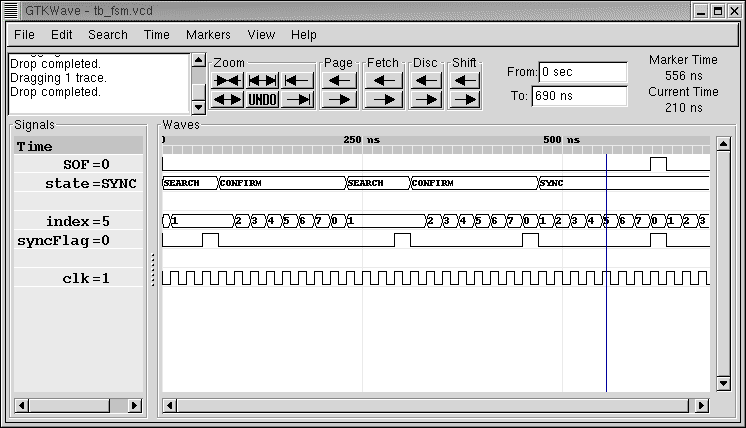
\includegraphics{tbfsm.png}
\fi


%======================================================================
\section{PEP 218: A Standard Set Datatype}

The new \module{sets} module contains an implementation of a set
datatype.  The \class{Set} class is for mutable sets, sets that can
have members added and removed.  The \class{ImmutableSet} class is for
sets that can't be modified, and instances of \class{ImmutableSet} can
therefore be used as dictionary keys.  Sets are built on top of
dictionaries, so the elements within a set must be hashable.

Here's a simple example:

\begin{verbatim}
>>> import sets
>>> S = sets.Set([1,2,3])
>>> S
Set([1, 2, 3])
>>> 1 in S
True
>>> 0 in S
False
>>> S.add(5)
>>> S.remove(3)
>>> S
Set([1, 2, 5])
>>>
\end{verbatim}

The union and intersection of sets can be computed with the
\method{union()} and \method{intersection()} methods or
alternatively using the bitwise operators \code{\&} and \code{|}.
Mutable sets also have in-place versions of these methods,
\method{union_update()} and \method{intersection_update()}.

\begin{verbatim}
>>> S1 = sets.Set([1,2,3])
>>> S2 = sets.Set([4,5,6])
>>> S1.union(S2)
Set([1, 2, 3, 4, 5, 6])
>>> S1 | S2                  # Alternative notation
Set([1, 2, 3, 4, 5, 6])
>>> S1.intersection(S2)
Set([])
>>> S1 & S2                  # Alternative notation
Set([])
>>> S1.union_update(S2)
>>> S1
Set([1, 2, 3, 4, 5, 6])
>>>
\end{verbatim}

It's also possible to take the symmetric difference of two sets.  This
is the set of all elements in the union that aren't in the
intersection.  An alternative way of expressing the symmetric
difference is that it contains all elements that are in exactly one
set.  Again, there's an alternative notation (\code{\^}), and an
in-place version with the ungainly name
\method{symmetric_difference_update()}.

\begin{verbatim}
>>> S1 = sets.Set([1,2,3,4])
>>> S2 = sets.Set([3,4,5,6])
>>> S1.symmetric_difference(S2)
Set([1, 2, 5, 6])
>>> S1 ^ S2
Set([1, 2, 5, 6])
>>>
\end{verbatim}

There are also \method{issubset()} and \method{issuperset()} methods
for checking whether one set is a subset or superset of another:

\begin{verbatim}
>>> S1 = sets.Set([1,2,3])
>>> S2 = sets.Set([2,3])
>>> S2.issubset(S1)
True
>>> S1.issubset(S2)
False
>>> S1.issuperset(S2)
True
>>>
\end{verbatim}


\begin{seealso}

\seepep{218}{Adding a Built-In Set Object Type}{PEP written by Greg V. Wilson.
Implemented by Greg V. Wilson, Alex Martelli, and GvR.}

\end{seealso}



%======================================================================
\section{PEP 255: Simple Generators\label{section-generators}}

In Python 2.2, generators were added as an optional feature, to be
enabled by a \code{from __future__ import generators} directive.  In
2.3 generators no longer need to be specially enabled, and are now
always present; this means that \keyword{yield} is now always a
keyword.  The rest of this section is a copy of the description of
generators from the ``What's New in Python 2.2'' document; if you read
it back when Python 2.2 came out, you can skip the rest of this section.

You're doubtless familiar with how function calls work in Python or C.
When you call a function, it gets a private namespace where its local
variables are created.  When the function reaches a \keyword{return}
statement, the local variables are destroyed and the resulting value
is returned to the caller.  A later call to the same function will get
a fresh new set of local variables. But, what if the local variables
weren't thrown away on exiting a function?  What if you could later
resume the function where it left off?  This is what generators
provide; they can be thought of as resumable functions.

Here's the simplest example of a generator function:

\begin{verbatim}
def generate_ints(N):
    for i in range(N):
        yield i
\end{verbatim}

A new keyword, \keyword{yield}, was introduced for generators.  Any
function containing a \keyword{yield} statement is a generator
function; this is detected by Python's bytecode compiler which
compiles the function specially as a result.

When you call a generator function, it doesn't return a single value;
instead it returns a generator object that supports the iterator
protocol.  On executing the \keyword{yield} statement, the generator
outputs the value of \code{i}, similar to a \keyword{return}
statement.  The big difference between \keyword{yield} and a
\keyword{return} statement is that on reaching a \keyword{yield} the
generator's state of execution is suspended and local variables are
preserved.  On the next call to the generator's \code{.next()} method,
the function will resume executing immediately after the
\keyword{yield} statement.  (For complicated reasons, the
\keyword{yield} statement isn't allowed inside the \keyword{try} block
of a \keyword{try}...\keyword{finally} statement; read \pep{255} for a full
explanation of the interaction between \keyword{yield} and
exceptions.)

Here's a sample usage of the \function{generate_ints()} generator:

\begin{verbatim}
>>> gen = generate_ints(3)
>>> gen
<generator object at 0x8117f90>
>>> gen.next()
0
>>> gen.next()
1
>>> gen.next()
2
>>> gen.next()
Traceback (most recent call last):
  File "stdin", line 1, in ?
  File "stdin", line 2, in generate_ints
StopIteration
\end{verbatim}

You could equally write \code{for i in generate_ints(5)}, or
\code{a,b,c = generate_ints(3)}.

Inside a generator function, the \keyword{return} statement can only
be used without a value, and signals the end of the procession of
values; afterwards the generator cannot return any further values.
\keyword{return} with a value, such as \code{return 5}, is a syntax
error inside a generator function.  The end of the generator's results
can also be indicated by raising \exception{StopIteration} manually,
or by just letting the flow of execution fall off the bottom of the
function.

You could achieve the effect of generators manually by writing your
own class and storing all the local variables of the generator as
instance variables.  For example, returning a list of integers could
be done by setting \code{self.count} to 0, and having the
\method{next()} method increment \code{self.count} and return it.
However, for a moderately complicated generator, writing a
corresponding class would be much messier.
\file{Lib/test/test_generators.py} contains a number of more
interesting examples.  The simplest one implements an in-order
traversal of a tree using generators recursively.

\begin{verbatim}
# A recursive generator that generates Tree leaves in in-order.
def inorder(t):
    if t:
        for x in inorder(t.left):
            yield x
        yield t.label
        for x in inorder(t.right):
            yield x
\end{verbatim}

Two other examples in \file{Lib/test/test_generators.py} produce
solutions for the N-Queens problem (placing $N$ queens on an $NxN$
chess board so that no queen threatens another) and the Knight's Tour
(a route that takes a knight to every square of an $NxN$ chessboard
without visiting any square twice).

The idea of generators comes from other programming languages,
especially Icon (\url{http://www.cs.arizona.edu/icon/}), where the
idea of generators is central.  In Icon, every
expression and function call behaves like a generator.  One example
from ``An Overview of the Icon Programming Language'' at
\url{http://www.cs.arizona.edu/icon/docs/ipd266.htm} gives an idea of
what this looks like:

\begin{verbatim}
sentence := "Store it in the neighboring harbor"
if (i := find("or", sentence)) > 5 then write(i)
\end{verbatim}

In Icon the \function{find()} function returns the indexes at which the
substring ``or'' is found: 3, 23, 33.  In the \keyword{if} statement,
\code{i} is first assigned a value of 3, but 3 is less than 5, so the
comparison fails, and Icon retries it with the second value of 23.  23
is greater than 5, so the comparison now succeeds, and the code prints
the value 23 to the screen.

Python doesn't go nearly as far as Icon in adopting generators as a
central concept.  Generators are considered part of the core
Python language, but learning or using them isn't compulsory; if they
don't solve any problems that you have, feel free to ignore them.
One novel feature of Python's interface as compared to
Icon's is that a generator's state is represented as a concrete object
(the iterator) that can be passed around to other functions or stored
in a data structure.

\begin{seealso}

\seepep{255}{Simple Generators}{Written by Neil Schemenauer, Tim
Peters, Magnus Lie Hetland.  Implemented mostly by Neil Schemenauer
and Tim Peters, with other fixes from the Python Labs crew.}

\end{seealso}


%======================================================================
\section{PEP 263: Source Code Encodings \label{section-encodings}}

Python source files can now be declared as being in different
character set encodings.  Encodings are declared by including a
specially formatted comment in the first or second line of the source
file.  For example, a UTF-8 file can be declared with:

\begin{verbatim}
#!/usr/bin/env python
# -*- coding: UTF-8 -*-
\end{verbatim}

Without such an encoding declaration, the default encoding used is
7-bit ASCII.  Executing or importing modules containing string
literals with 8-bit characters and no encoding declaration will result
in a \exception{DeprecationWarning} being signalled by Python 2.3; in
2.4 this will be a syntax error.

The encoding declaration only affects Unicode string literals, which
will be converted to Unicode using the specified encoding.  Note that
Python identifiers are still restricted to ASCII characters, so you
can't have variable names that use characters outside of the usual
alphanumerics.

\begin{seealso}

\seepep{263}{Defining Python Source Code Encodings}{Written by
Marc-Andr\'e Lemburg and Martin von L\"owis; implemented by SUZUKI
Hisao and Martin von L\"owis.}

\end{seealso}


%======================================================================
\section{PEP 277: Unicode file name support for Windows NT}

On Windows NT, 2000, and XP, the system stores file names as Unicode
strings. Traditionally, Python has represented file names as byte
strings, which is inadequate because it renders some file names
inaccessible.

Python now allows using arbitrary Unicode strings (within the
limitations of the file system) for all functions that expect file
names, most notably the \function{open()} built-in function. If a Unicode
string is passed to \function{os.listdir()}, Python now returns a list
of Unicode strings.  A new function, \function{os.getcwdu()}, returns
the current directory as a Unicode string.

Byte strings still work as file names, and on Windows Python will
transparently convert them to Unicode using the \code{mbcs} encoding.

Other systems also allow Unicode strings as file names but convert
them to byte strings before passing them to the system, which can
cause a \exception{UnicodeError} to be raised. Applications can test
whether arbitrary Unicode strings are supported as file names by
checking \member{os.path.supports_unicode_filenames}, a Boolean value.

\begin{seealso}

\seepep{277}{Unicode file name support for Windows NT}{Written by Neil
Hodgson; implemented by Neil Hodgson, Martin von L\"owis, and Mark
Hammond.}

\end{seealso}


%======================================================================
\section{PEP 278: Universal Newline Support}

The three major operating systems used today are Microsoft Windows,
Apple's Macintosh OS, and the various \UNIX\ derivatives.  A minor
irritation is that these three platforms all use different characters
to mark the ends of lines in text files.  \UNIX\ uses the linefeed
(ASCII character 10), while MacOS uses the carriage return (ASCII
character 13), and Windows uses a two-character sequence containing a
carriage return plus a newline.

Python's file objects can now support end of line conventions other
than the one followed by the platform on which Python is running.
Opening a file with the mode \code{'U'} or \code{'rU'} will open a file
for reading in universal newline mode.  All three line ending
conventions will be translated to a \character{\e n} in the strings
returned by the various file methods such as \method{read()} and
\method{readline()}.

Universal newline support is also used when importing modules and when
executing a file with the \function{execfile()} function.  This means
that Python modules can be shared between all three operating systems
without needing to convert the line-endings.

This feature can be disabled at compile-time by specifying
\longprogramopt{without-universal-newlines} when running Python's
\program{configure} script.

\begin{seealso}

\seepep{278}{Universal Newline Support}{Written
and implemented by Jack Jansen.}

\end{seealso}


%======================================================================
\section{PEP 279: The \function{enumerate()} Built-in Function\label{section-enumerate}}

A new built-in function, \function{enumerate()}, will make
certain loops a bit clearer.  \code{enumerate(thing)}, where
\var{thing} is either an iterator or a sequence, returns a iterator
that will return \code{(0, \var{thing[0]})}, \code{(1,
\var{thing[1]})}, \code{(2, \var{thing[2]})}, and so forth.  

Fairly often you'll see code to change every element of a list that
looks like this:

\begin{verbatim}
for i in range(len(L)):
    item = L[i]
    # ... compute some result based on item ...
    L[i] = result
\end{verbatim}

This can be rewritten using \function{enumerate()} as:

\begin{verbatim}
for i, item in enumerate(L):
    # ... compute some result based on item ...
    L[i] = result
\end{verbatim}


\begin{seealso}

\seepep{279}{The enumerate() built-in function}{Written
and implemented by Raymond D. Hettinger.}

\end{seealso}


%======================================================================
\section{PEP 282: The \module{logging} Package}

A standard package for writing logs, \module{logging}, has been added
to Python 2.3.  It provides a powerful and flexible mechanism for
components to generate logging output which can then be filtered and
processed in various ways.  A standard configuration file format can
be used to control the logging behavior of a program.  Python's
standard library includes handlers that will write log records to
standard error or to a file or socket, send them to the system log, or
even e-mail them to a particular address, and of course it's also
possible to write your own handler classes.

The \class{Logger} class is the primary class.
Most application code will deal with one or more \class{Logger}
objects, each one used by a particular subsystem of the application.
Each \class{Logger} is identified by a name, and names are organized
into a hierarchy using \samp{.}  as the component separator.  For
example, you might have \class{Logger} instances named \samp{server},
\samp{server.auth} and \samp{server.network}.  The latter two
instances are below \samp{server} in the hierarchy.  This means that
if you turn up the verbosity for \samp{server} or direct \samp{server}
messages to a different handler, the changes will also apply to
records logged to \samp{server.auth} and \samp{server.network}.
There's also a root \class{Logger} that's the parent of all other
loggers.

For simple uses, the \module{logging} package contains some
convenience functions that always use the root log:

\begin{verbatim}
import logging

logging.debug('Debugging information')
logging.info('Informational message')
logging.warning('Warning:config file %s not found', 'server.conf')
logging.error('Error occurred')
logging.critical('Critical error -- shutting down')
\end{verbatim}

This produces the following output:

\begin{verbatim}
WARNING:root:Warning:config file server.conf not found
ERROR:root:Error occurred
CRITICAL:root:Critical error -- shutting down
\end{verbatim}

In the default configuration, informational and debugging messages are
suppressed and the output is sent to standard error.  You can enable
the display of information and debugging messages by calling the
\method{setLevel()} method on the root logger.

Notice the \function{warning()} call's use of string formatting
operators; all of the functions for logging messages take the
arguments \code{(\var{msg}, \var{arg1}, \var{arg2}, ...)} and log the
string resulting from \code{\var{msg} \% (\var{arg1}, \var{arg2},
...)}.

There's also an \function{exception()} function that records the most
recent traceback.  Any of the other functions will also record the
traceback if you specify a true value for the keyword argument
\var{exc_info}.

\begin{verbatim}
def f():
    try:    1/0
    except: logging.exception('Problem recorded')

f()
\end{verbatim}

This produces the following output:

\begin{verbatim}
ERROR:root:Problem recorded
Traceback (most recent call last):
  File "t.py", line 6, in f
    1/0
ZeroDivisionError: integer division or modulo by zero
\end{verbatim}

Slightly more advanced programs will use a logger other than the root
logger.  The \function{getLogger(\var{name})} function is used to get
a particular log, creating it if it doesn't exist yet.
\function{getLogger(None)} returns the root logger.


\begin{verbatim}
log = logging.getLogger('server')
 ...
log.info('Listening on port %i', port)
 ...
log.critical('Disk full')
 ...
\end{verbatim}

Log records are usually propagated up the hierarchy, so a message
logged to \samp{server.auth} is also seen by \samp{server} and
\samp{root}, but a handler can prevent this by setting its
\member{propagate} attribute to \constant{False}.

There are more classes provided by the \module{logging} package that
can be customized.  When a \class{Logger} instance is told to log a
message, it creates a \class{LogRecord} instance that is sent to any
number of different \class{Handler} instances.  Loggers and handlers
can also have an attached list of filters, and each filter can cause
the \class{LogRecord} to be ignored or can modify the record before
passing it along.  \class{LogRecord} instances are converted to text
for output by a \class{Formatter} class.  All of these classes can be
replaced by your own specially-written classes.

With all of these features the \module{logging} package should provide
enough flexibility for even the most complicated applications.  This
is only a partial overview of the \module{logging} package, so please
see the \ulink{package's reference
documentation}{../lib/module-logging.html} for all of the details.
Reading \pep{282} will also be helpful.


\begin{seealso}

\seepep{282}{A Logging System}{Written by Vinay Sajip and Trent Mick;
implemented by Vinay Sajip.}

\end{seealso}


%======================================================================
\section{PEP 285: The \class{bool} Type\label{section-bool}}

A Boolean type was added to Python 2.3.  Two new constants were added
to the \module{__builtin__} module, \constant{True} and
\constant{False}.  (\constant{True} and
\constant{False} constants were added to the built-ins
in Python 2.2.1, but the 2.2.1 versions simply have integer values of
1 and 0 and aren't a different type.)

The type object for this new type is named
\class{bool}; the constructor for it takes any Python value and
converts it to \constant{True} or \constant{False}.

\begin{verbatim}
>>> bool(1)
True
>>> bool(0)
False
>>> bool([])
False
>>> bool( (1,) )
True
\end{verbatim}

Most of the standard library modules and built-in functions have been
changed to return Booleans.

\begin{verbatim}
>>> obj = []
>>> hasattr(obj, 'append')
True
>>> isinstance(obj, list)
True
>>> isinstance(obj, tuple)
False
\end{verbatim}

Python's Booleans were added with the primary goal of making code
clearer.  For example, if you're reading a function and encounter the
statement \code{return 1}, you might wonder whether the \code{1}
represents a Boolean truth value, an index, or a
coefficient that multiplies some other quantity.  If the statement is
\code{return True}, however, the meaning of the return value is quite
clear.

Python's Booleans were \emph{not} added for the sake of strict
type-checking.  A very strict language such as Pascal would also
prevent you performing arithmetic with Booleans, and would require
that the expression in an \keyword{if} statement always evaluate to a
Boolean.  Python is not this strict, and it never will be, as
\pep{285} explicitly says.  This means you can still use any
expression in an \keyword{if} statement, even ones that evaluate to a
list or tuple or some random object, and the Boolean type is a
subclass of the \class{int} class so that arithmetic using a Boolean
still works.

\begin{verbatim}
>>> True + 1
2
>>> False + 1
1
>>> False * 75
0
>>> True * 75
75
\end{verbatim}

To sum up \constant{True} and \constant{False} in a sentence: they're
alternative ways to spell the integer values 1 and 0, with the single
difference that \function{str()} and \function{repr()} return the
strings \code{'True'} and \code{'False'} instead of \code{'1'} and
\code{'0'}.

\begin{seealso}

\seepep{285}{Adding a bool type}{Written and implemented by GvR.}

\end{seealso}


%======================================================================
\section{PEP 293: Codec Error Handling Callbacks}

When encoding a Unicode string into a byte string, unencodable
characters may be encountered.  So far, Python has allowed specifying
the error processing as either ``strict'' (raising
\exception{UnicodeError}), ``ignore'' (skipping the character), or
``replace'' (using a question mark in the output string), with
``strict'' being the default behavior. It may be desirable to specify
alternative processing of such errors, such as inserting an XML
character reference or HTML entity reference into the converted
string.

Python now has a flexible framework to add different processing
strategies.  New error handlers can be added with
\function{codecs.register_error}. Codecs then can access the error
handler with \function{codecs.lookup_error}. An equivalent C API has
been added for codecs written in C. The error handler gets the
necessary state information such as the string being converted, the
position in the string where the error was detected, and the target
encoding.  The handler can then either raise an exception or return a
replacement string.

Two additional error handlers have been implemented using this
framework: ``backslashreplace'' uses Python backslash quoting to
represent unencodable characters and ``xmlcharrefreplace'' emits
XML character references.

\begin{seealso}

\seepep{293}{Codec Error Handling Callbacks}{Written and implemented by
Walter D\"orwald.}

\end{seealso}


%======================================================================
\section{PEP 273: Importing Modules from Zip Archives}

The new \module{zipimport} module adds support for importing
modules from a ZIP-format archive.  You don't need to import the
module explicitly; it will be automatically imported if a ZIP
archive's filename is added to \code{sys.path}.  For example:

\begin{verbatim}
amk@nyman:~/src/python$ unzip -l /tmp/example.zip
Archive:  /tmp/example.zip
  Length     Date   Time    Name
 --------    ----   ----    ----
     8467  11-26-02 22:30   jwzthreading.py
 --------                   -------
     8467                   1 file
amk@nyman:~/src/python$ ./python
Python 2.3a0 (#1, Dec 30 2002, 19:54:32) 
>>> import sys
>>> sys.path.insert(0, '/tmp/example.zip')  # Add .zip file to front of path
>>> import jwzthreading
>>> jwzthreading.__file__
'/tmp/example.zip/jwzthreading.py'
>>>
\end{verbatim}

An entry in \code{sys.path} can now be the filename of a ZIP archive.
The ZIP archive can contain any kind of files, but only files named
\file{*.py}, \file{*.pyc}, or \file{*.pyo} can be imported.  If an
archive only contains \file{*.py} files, Python will not attempt to
modify the archive by adding the corresponding \file{*.pyc} file, meaning
that if a ZIP archive doesn't contain \file{*.pyc} files, importing may be
rather slow.

A path within the archive can also be specified to only import from a
subdirectory; for example, the path \file{/tmp/example.zip/lib/}
would only import from the \file{lib/} subdirectory within the
archive.

\begin{seealso}

\seepep{273}{Import Modules from Zip Archives}{Written by James C. Ahlstrom, 
who also provided an implementation.
Python 2.3 follows the specification in \pep{273}, 
but uses an implementation written by Just van~Rossum 
that uses the import hooks described in \pep{302}.
See section~\ref{section-pep302} for a description of the new import hooks.
}

\end{seealso}

%======================================================================
\section{PEP 301: Package Index and Metadata for
Distutils\label{section-pep301}}

Support for the long-requested Python catalog makes its first
appearance in 2.3.

The core component is the new Distutils \command{register} command.
Running \code{python setup.py register} will collect the metadata
describing a package, such as its name, version, maintainer,
description, \&c., and send it to a central catalog server.
Currently the catalog can be browsed at
\url{http://www.amk.ca/cgi-bin/pypi.cgi}, but it will move to 
some hostname in the \code{python.org} domain before the final version
of 2.3 is released.

To make the catalog a bit more useful, a new optional
\var{classifiers} keyword argument has been added to the Distutils
\function{setup()} function.  A list of
\ulink{Trove}{http://catb.org/\textasciitilde esr/trove/}-style
strings can be supplied to help classify the software.

Here's an example \file{setup.py} with classifiers, written to be compatible 
with older versions of the Distutils:

\begin{verbatim}
from distutils import core
kw = {'name': "Quixote",
      'version': "0.5.1",
      'description': "A highly Pythonic Web application framework",
      # ...
      }

if (  hasattr(core, 'setup_keywords') and 
      'classifiers' in core.setup_keywords):
    kw['classifiers'] = \
        ['Topic :: Internet :: WWW/HTTP :: Dynamic Content',
         'Environment :: No Input/Output (Daemon)',
         'Intended Audience :: Developers'],

core.setup(**kw)
\end{verbatim}

The full list of classifiers can be obtained by running 
\code{python setup.py register --list-classifiers}.

\begin{seealso}

\seepep{301}{Package Index and Metadata for Distutils}{Written and
implemented by Richard Jones.}

\end{seealso}


%======================================================================
\section{PEP 302: New Import Hooks \label{section-pep302}}

While it's been possible to write custom import hooks ever since the
\module{ihooks} module was introduced in Python 1.3, no one has ever
been really happy with it because writing new import hooks is
difficult and messy.  There have been various proposed alternatives
such as the \module{imputil} and \module{iu} modules, but none of them
has ever gained much acceptance, and none of them were easily usable
from \C{} code.

\pep{302} borrows ideas from its predecessors, especially from
Gordon McMillan's \module{iu} module.  Three new items 
are added to the \module{sys} module:

\begin{itemize}
  \item \code{sys.path_hooks} is a list of callable objects; most 
  often they'll be classes.  Each callable takes a string containing a
  path and either returns an importer object that will handle imports
  from this path or raises an \exception{ImportError} exception if it
  can't handle this path.

  \item \code{sys.path_importer_cache} caches importer objects for
  each path, so \code{sys.path_hooks} will only need to be traversed
  once for each path.

  \item \code{sys.meta_path} is a list of importer objects that will
  be traversed before \code{sys.path} is checked.  This list is
  initially empty, but user code can add objects to it.  Additional
  built-in and frozen modules can be imported by an object added to
  this list.

\end{itemize}

Importer objects must have a single method,
\method{find_module(\var{fullname}, \var{path}=None)}.  \var{fullname}
will be a module or package name, e.g. \samp{string} or
\samp{distutils.core}.  \method{find_module()} must return a loader object
that has a single method, \method{load_module(\var{fullname})}, that
creates and returns the corresponding module object.

Pseudo-code for Python's new import logic, therefore, looks something
like this (simplified a bit; see \pep{302} for the full details):

\begin{verbatim}
for mp in sys.meta_path:
    loader = mp(fullname)
    if loader is not None:
        <module> = loader.load_module(fullname)
        
for path in sys.path:
    for hook in sys.path_hooks:
        try:
            importer = hook(path)
        except ImportError:
            # ImportError, so try the other path hooks
            pass
        else:
            loader = importer.find_module(fullname)
            <module> = loader.load_module(fullname)

# Not found!
raise ImportError
\end{verbatim}

\begin{seealso}

\seepep{302}{New Import Hooks}{Written by Just van~Rossum and Paul Moore.
Implemented by Just van~Rossum.
}

\end{seealso}


%======================================================================
\section{Extended Slices\label{section-slices}}

Ever since Python 1.4, the slicing syntax has supported an optional
third ``step'' or ``stride'' argument.  For example, these are all
legal Python syntax: \code{L[1:10:2]}, \code{L[:-1:1]},
\code{L[::-1]}.  This was added to Python at the request of
the developers of Numerical Python, which uses the third argument
extensively.  However, Python's built-in list, tuple, and string
sequence types have never supported this feature, and you got a
\exception{TypeError} if you tried it.  Michael Hudson contributed a
patch to fix this shortcoming.

For example, you can now easily extract the elements of a list that
have even indexes:

\begin{verbatim}
>>> L = range(10)
>>> L[::2]
[0, 2, 4, 6, 8]
\end{verbatim}

Negative values also work to make a copy of the same list in reverse
order:

\begin{verbatim}
>>> L[::-1]
[9, 8, 7, 6, 5, 4, 3, 2, 1, 0]
\end{verbatim}

This also works for tuples, arrays, and strings:

\begin{verbatim}
>>> s='abcd'
>>> s[::2]
'ac'
>>> s[::-1]
'dcba'
\end{verbatim}

If you have a mutable sequence such as a list or an array you can
assign to or delete an extended slice, but there are some differences
between assignment to extended and regular slices.  Assignment to a
regular slice can be used to change the length of the sequence:

\begin{verbatim}
>>> a = range(3)
>>> a
[0, 1, 2]
>>> a[1:3] = [4, 5, 6]
>>> a
[0, 4, 5, 6]
\end{verbatim}

Extended slices aren't this flexible.  When assigning to an extended
slice the list on the right hand side of the statement must contain
the same number of items as the slice it is replacing:

\begin{verbatim}
>>> a = range(4)
>>> a
[0, 1, 2, 3]
>>> a[::2]
[0, 2]
>>> a[::2] = [0, -1]
>>> a
[0, 1, -1, 3]
>>> a[::2] = [0,1,2]
Traceback (most recent call last):
  File "<stdin>", line 1, in ?
ValueError: attempt to assign sequence of size 3 to extended slice of size 2
\end{verbatim}

Deletion is more straightforward:

\begin{verbatim}
>>> a = range(4)
>>> a
[0, 1, 2, 3]
>>> a[::2]
[0, 2]
>>> del a[::2]
>>> a
[1, 3]
\end{verbatim}

One can also now pass slice objects to the
\method{__getitem__} methods of the built-in sequences:

\begin{verbatim}
>>> range(10).__getitem__(slice(0, 5, 2))
[0, 2, 4]
\end{verbatim}

Or use slice objects directly in subscripts:

\begin{verbatim}
>>> range(10)[slice(0, 5, 2)]
[0, 2, 4]
\end{verbatim}

To simplify implementing sequences that support extended slicing,
slice objects now have a method \method{indices(\var{length})} which,
given the length of a sequence, returns a \code{(\var{start},
\var{stop}, \var{step})} tuple that can be passed directly to
\function{range()}.
\method{indices()} handles omitted and out-of-bounds indices in a
manner consistent with regular slices (and this innocuous phrase hides
a welter of confusing details!).  The method is intended to be used
like this:

\begin{verbatim}
class FakeSeq:
    ...
    def calc_item(self, i):
        ...
    def __getitem__(self, item):
        if isinstance(item, slice):
            indices = item.indices(len(self))
            return FakeSeq([self.calc_item(i) in range(*indices)])
        else:
            return self.calc_item(i)
\end{verbatim}

From this example you can also see that the built-in \class{slice}
object is now the type object for the slice type, and is no longer a
function.  This is consistent with Python 2.2, where \class{int},
\class{str}, etc., underwent the same change.


%======================================================================
\section{Other Language Changes}

Here are all of the changes that Python 2.3 makes to the core Python
language.

\begin{itemize}
\item The \keyword{yield} statement is now always a keyword, as
described in section~\ref{section-generators} of this document.

\item A new built-in function \function{enumerate()}
was added, as described in section~\ref{section-enumerate} of this
document.

\item Two new constants, \constant{True} and \constant{False} were
added along with the built-in \class{bool} type, as described in
section~\ref{section-bool} of this document.

\item The \function{int()} type constructor will now return a long
integer instead of raising an \exception{OverflowError} when a string
or floating-point number is too large to fit into an integer.  This
can lead to the paradoxical result that
\code{isinstance(int(\var{expression}), int)} is false, but that seems
unlikely to cause problems in practice.

\item Built-in types now support the extended slicing syntax,
as described in section~\ref{section-slices} of this document.

\item Dictionaries have a new method, \method{pop(\var{key})}, that
returns the value corresponding to \var{key} and removes that
key/value pair from the dictionary.  \method{pop()} will raise a
\exception{KeyError} if the requested key isn't present in the
dictionary:

\begin{verbatim}
>>> d = {1:2}
>>> d
{1: 2}
>>> d.pop(4)
Traceback (most recent call last):
  File "stdin", line 1, in ?
KeyError: 4
>>> d.pop(1)
2
>>> d.pop(1)
Traceback (most recent call last):
  File "stdin", line 1, in ?
KeyError: 'pop(): dictionary is empty'
>>> d
{}
>>>
\end{verbatim}

There's also a new class method, 
\method{dict.fromkeys(\var{iterable}, \var{value})}, that 
creates a dictionary with keys taken from the supplied iterator
\var{iterable} and all values set to \var{value}, defaulting to
\code{None}.  

(Patches contributed by Raymond Hettinger.)

Also, the \function{dict()} constructor now accepts keyword arguments to
simplify creating small dictionaries:

\begin{verbatim}
>>> dict(red=1, blue=2, green=3, black=4)
{'blue': 2, 'black': 4, 'green': 3, 'red': 1}    
\end{verbatim}

(Contributed by Just van~Rossum.)       

\item The \keyword{assert} statement no longer checks the \code{__debug__}
flag, so you can no longer disable assertions by assigning to \code{__debug__}.
Running Python with the \programopt{-O} switch will still generate
code that doesn't execute any assertions.

\item Most type objects are now callable, so you can use them
to create new objects such as functions, classes, and modules.  (This
means that the \module{new} module can be deprecated in a future
Python version, because you can now use the type objects available in
the \module{types} module.)
% XXX should new.py use PendingDeprecationWarning?
For example, you can create a new module object with the following code:

\begin{verbatim}
>>> import types
>>> m = types.ModuleType('abc','docstring')
>>> m
<module 'abc' (built-in)>
>>> m.__doc__
'docstring'
\end{verbatim}

\item
A new warning, \exception{PendingDeprecationWarning} was added to
indicate features which are in the process of being
deprecated.  The warning will \emph{not} be printed by default.  To
check for use of features that will be deprecated in the future,
supply \programopt{-Walways::PendingDeprecationWarning::} on the
command line or use \function{warnings.filterwarnings()}.

\item The process of deprecating string-based exceptions, as
in \code{raise "Error occurred"}, has begun.  Raising a string will
now trigger \exception{PendingDeprecationWarning}.

\item Using \code{None} as a variable name will now result in a
\exception{SyntaxWarning} warning.  In a future version of Python,
\code{None} may finally become a keyword.

\item The method resolution order used by new-style classes has
changed, though you'll only notice the difference if you have a really
complicated inheritance hierarchy.  (Classic classes are unaffected by
this change.)  Python 2.2 originally used a topological sort of a
class's ancestors, but 2.3 now uses the C3 algorithm as described in
the paper \ulink{``A Monotonic Superclass Linearization for
Dylan''}{http://www.webcom.com/haahr/dylan/linearization-oopsla96.html}.
To understand the motivation for this change, 
read Michele Simionato's article 
\ulink{``Python 2.3 Method Resolution Order''}
      {http://www.python.org/2.3/mro.html}, or
read the thread on python-dev starting with the message at
\url{http://mail.python.org/pipermail/python-dev/2002-October/029035.html}.
Samuele Pedroni first pointed out the problem and also implemented the
fix by coding the C3 algorithm.

\item Python runs multithreaded programs by switching between threads
after executing N bytecodes.  The default value for N has been
increased from 10 to 100 bytecodes, speeding up single-threaded
applications by reducing the switching overhead.  Some multithreaded
applications may suffer slower response time, but that's easily fixed
by setting the limit back to a lower number using
\function{sys.setcheckinterval(\var{N})}.

\item One minor but far-reaching change is that the names of extension
types defined by the modules included with Python now contain the
module and a \character{.} in front of the type name.  For example, in
Python 2.2, if you created a socket and printed its
\member{__class__}, you'd get this output:

\begin{verbatim}
>>> s = socket.socket()
>>> s.__class__
<type 'socket'>
\end{verbatim}

In 2.3, you get this:
\begin{verbatim}
>>> s.__class__
<type '_socket.socket'>
\end{verbatim}

\item One of the noted incompatibilities between old- and new-style
  classes has been removed: you can now assign to the
  \member{__name__} and \member{__bases__} attributes of new-style
  classes.  There are some restrictions on what can be assigned to
  \member{__bases__} along the lines of those relating to assigning to
  an instance's \member{__class__} attribute.

\end{itemize}


%======================================================================
\subsection{String Changes}

\begin{itemize}

\item The \keyword{in} operator now works differently for strings.
Previously, when evaluating \code{\var{X} in \var{Y}} where \var{X}
and \var{Y} are strings, \var{X} could only be a single character.
That's now changed; \var{X} can be a string of any length, and
\code{\var{X} in \var{Y}} will return \constant{True} if \var{X} is a
substring of \var{Y}.  If \var{X} is the empty string, the result is
always \constant{True}.

\begin{verbatim}
>>> 'ab' in 'abcd'
True
>>> 'ad' in 'abcd'
False
>>> '' in 'abcd'
True
\end{verbatim}

Note that this doesn't tell you where the substring starts; if you
need that information, you must use the \method{find()} method
instead.

\item The \method{strip()}, \method{lstrip()}, and \method{rstrip()}
string methods now have an optional argument for specifying the
characters to strip.  The default is still to remove all whitespace
characters:

\begin{verbatim}
>>> '   abc '.strip()
'abc'
>>> '><><abc<><><>'.strip('<>')
'abc'
>>> '><><abc<><><>\n'.strip('<>')
'abc<><><>\n'
>>> u'\u4000\u4001abc\u4000'.strip(u'\u4000')
u'\u4001abc'
>>>
\end{verbatim}

(Suggested by Simon Brunning and implemented by Walter D\"orwald.)

\item The \method{startswith()} and \method{endswith()}
string methods now accept negative numbers for the start and end
parameters.

\item Another new string method is \method{zfill()}, originally a
function in the \module{string} module.  \method{zfill()} pads a
numeric string with zeros on the left until it's the specified width.
Note that the \code{\%} operator is still more flexible and powerful
than \method{zfill()}.

\begin{verbatim}
>>> '45'.zfill(4)
'0045'
>>> '12345'.zfill(4)
'12345'
>>> 'goofy'.zfill(6)
'0goofy'
\end{verbatim}

(Contributed by Walter D\"orwald.)

\item A new type object, \class{basestring}, has been added.
   Both 8-bit strings and Unicode strings inherit from this type, so
   \code{isinstance(obj, basestring)} will return \constant{True} for
   either kind of string.  It's a completely abstract type, so you
   can't create \class{basestring} instances.

\item Interned strings are no longer immortal, and will now be
garbage-collected in the usual way when the only reference to them is
from the internal dictionary of interned strings.  (Implemented by
Oren Tirosh.)

\end{itemize}


%======================================================================
\subsection{Optimizations}

\begin{itemize}

\item The creation of new-style class instances has been made much
faster; they're now faster than classic classes!

\item The \method{sort()} method of list objects has been extensively
rewritten by Tim Peters, and the implementation is significantly
faster.

\item Multiplication of large long integers is now much faster thanks
to an implementation of Karatsuba multiplication, an algorithm that
scales better than the O(n*n) required for the grade-school
multiplication algorithm.  (Original patch by Christopher A. Craig,
and significantly reworked by Tim Peters.)

\item The \code{SET_LINENO} opcode is now gone.  This may provide a
small speed increase, depending on your compiler's idiosyncrasies.
See section~\ref{section-other} for a longer explanation.
(Removed by Michael Hudson.)

\item \function{xrange()} objects now have their own iterator, making
\code{for i in xrange(n)} slightly faster than
\code{for i in range(n)}.  (Patch by Raymond Hettinger.)

\item A number of small rearrangements have been made in various
hotspots to improve performance, inlining a function here, removing
some code there.  (Implemented mostly by GvR, but lots of people have
contributed single changes.)

\end{itemize}


%======================================================================
\section{New, Improved, and Deprecated Modules}

As usual, Python's standard library received a number of enhancements and
bug fixes.  Here's a partial list of the most notable changes, sorted
alphabetically by module name. Consult the
\file{Misc/NEWS} file in the source tree for a more
complete list of changes, or look through the CVS logs for all the
details.

\begin{itemize}

\item The \module{array} module now supports arrays of Unicode
characters using the \character{u} format character.  Arrays also now
support using the \code{+=} assignment operator to add another array's
contents, and the \code{*=} assignment operator to repeat an array.
(Contributed by Jason Orendorff.)

\item The \module{bsddb} module has been replaced by version 4.1.1
of the \ulink{PyBSDDB}{http://pybsddb.sourceforge.net} package,
providing a more complete interface to the transactional features of
the BerkeleyDB library.
The old version of the module has been renamed to 
\module{bsddb185} and is no longer built automatically; you'll 
have to edit \file{Modules/Setup} to enable it.  Note that the new
\module{bsddb} package is intended to be compatible with the 
old module, so be sure to file bugs if you discover any
incompatibilities.
 
\item The Distutils \class{Extension} class now supports
an extra constructor argument named \var{depends} for listing
additional source files that an extension depends on.  This lets
Distutils recompile the module if any of the dependency files are
modified.  For example, if \file{sampmodule.c} includes the header
file \file{sample.h}, you would create the \class{Extension} object like
this:

\begin{verbatim}
ext = Extension("samp",
                sources=["sampmodule.c"],
                depends=["sample.h"])
\end{verbatim}

Modifying \file{sample.h} would then cause the module to be recompiled.
(Contributed by Jeremy Hylton.)

\item Other minor changes to Distutils:
it now checks for the \envvar{CC}, \envvar{CFLAGS}, \envvar{CPP},
\envvar{LDFLAGS}, and \envvar{CPPFLAGS} environment variables, using
them to override the settings in Python's configuration (contributed
by Robert Weber).

\item The \module{getopt} module gained a new function,
\function{gnu_getopt()}, that supports the same arguments as the existing
\function{getopt()} function but uses GNU-style scanning mode.
The existing \function{getopt()} stops processing options as soon as a
non-option argument is encountered, but in GNU-style mode processing
continues, meaning that options and arguments can be mixed.  For
example:

\begin{verbatim}
>>> getopt.getopt(['-f', 'filename', 'output', '-v'], 'f:v')
([('-f', 'filename')], ['output', '-v'])
>>> getopt.gnu_getopt(['-f', 'filename', 'output', '-v'], 'f:v')
([('-f', 'filename'), ('-v', '')], ['output'])
\end{verbatim}

(Contributed by Peter \AA{strand}.)

\item The \module{grp}, \module{pwd}, and \module{resource} modules
now return enhanced tuples:

\begin{verbatim}
>>> import grp
>>> g = grp.getgrnam('amk')
>>> g.gr_name, g.gr_gid
('amk', 500)
\end{verbatim}

\item The \module{gzip} module can now handle files exceeding 2~Gb.  

\item The new \module{heapq} module contains an implementation of a
heap queue algorithm.  A heap is an array-like data structure that
keeps items in a partially sorted order such that, for every index
\var{k}, \code{heap[\var{k}] <= heap[2*\var{k}+1]} and
\code{heap[\var{k}] <= heap[2*\var{k}+2]}.  This makes it quick to
remove the smallest item, and inserting a new item while maintaining
the heap property is O(lg~n).  (See
\url{http://www.nist.gov/dads/HTML/priorityque.html} for more
information about the priority queue data structure.)

The \module{heapq} module provides \function{heappush()} and
\function{heappop()} functions for adding and removing items while
maintaining the heap property on top of some other mutable Python
sequence type.  For example:

\begin{verbatim}
>>> import heapq
>>> heap = []
>>> for item in [3, 7, 5, 11, 1]:
...    heapq.heappush(heap, item)
...
>>> heap
[1, 3, 5, 11, 7]
>>> heapq.heappop(heap)
1
>>> heapq.heappop(heap)
3
>>> heap
[5, 7, 11]
\end{verbatim}

(Contributed by Kevin O'Connor.)

\item The \module{imaplib} module now supports IMAP over SSL.
(Contributed by Piers Lauder and Tino Lange.)

\item The \ulink{\module{itertools}}{../lib/module-itertools.html}
module provides several functions to support efficient looping using
iterators.

\item Two new functions in the \module{math} module,
\function{degrees(\var{rads})} and \function{radians(\var{degs})},
convert between radians and degrees.  Other functions in the
\module{math} module such as \function{math.sin()} and
\function{math.cos()} have always required input values measured in
radians.  Also, an optional \var{base} argument was added to
\function{math.log()} to make it easier to compute logarithms for
bases other than \code{e} and \code{10}.  (Contributed by Raymond
Hettinger.)

\item Several new functions (\function{getpgid()}, \function{killpg()},
\function{lchown()}, \function{loadavg()}, \function{major()}, \function{makedev()},
\function{minor()}, and \function{mknod()}) were added to the
\module{posix} module that underlies the \module{os} module.
(Contributed by Gustavo Niemeyer, Geert Jansen, and Denis S. Otkidach.)

\item In the \module{os} module, the \function{*stat()} family of functions can now report
fractions of a second in a timestamp.  Such time stamps are
represented as floats, similar to \function{time.time()}.

During testing, it was found that some applications will break if time
stamps are floats.  For compatibility, when using the tuple interface
of the \class{stat_result} time stamps will be represented as integers.
When using named fields (a feature first introduced in Python 2.2),
time stamps are still represented as integers, unless
\function{os.stat_float_times()} is invoked to enable float return
values:

\begin{verbatim}
>>> os.stat("/tmp").st_mtime
1034791200
>>> os.stat_float_times(True)
>>> os.stat("/tmp").st_mtime
1034791200.6335014
\end{verbatim}

In Python 2.4, the default will change to always returning floats.

Application developers should enable this feature only if all their
libraries work properly when confronted with floating point time
stamps, or if they use the tuple API. If used, the feature should be
activated on an application level instead of trying to enable it on a
per-use basis.

\item The old and never-documented \module{linuxaudiodev} module has
been deprecated, and a new version named \module{ossaudiodev} has been
added.  The module was renamed because the OSS sound drivers can be
used on platforms other than Linux, and the interface has also been
tidied and brought up to date in various ways. (Contributed by Greg
Ward and Nicholas FitzRoy-Dale.)

\item The parser objects provided by the \module{pyexpat} module
can now optionally buffer character data, resulting in fewer calls to
your character data handler and therefore faster performance.  Setting
the parser object's \member{buffer_text} attribute to \constant{True}
will enable buffering.

\item The \function{sample(\var{population}, \var{k})} function was
added to the \module{random} module.  \var{population} is a sequence
or \class{xrange} object containing the elements of a population, and
\function{sample()}
chooses \var{k} elements from the population without replacing chosen
elements.  \var{k} can be any value up to \code{len(\var{population})}.
For example:

\begin{verbatim}
>>> days = ['Mo', 'Tu', 'We', 'Th', 'Fr', 'St', 'Sn']
>>> random.sample(days, 3)      # Choose 3 elements
['St', 'Sn', 'Th']
>>> random.sample(days, 7)      # Choose 7 elements
['Tu', 'Th', 'Mo', 'We', 'St', 'Fr', 'Sn']
>>> random.sample(days, 7)      # Choose 7 again
['We', 'Mo', 'Sn', 'Fr', 'Tu', 'St', 'Th']
>>> random.sample(days, 8)      # Can't choose eight
Traceback (most recent call last):
  File "<stdin>", line 1, in ?
  File "random.py", line 414, in sample
      raise ValueError, "sample larger than population"
ValueError: sample larger than population
>>> random.sample(xrange(1,10000,2), 10)   # Choose ten odd nos. under 10000
[3407, 3805, 1505, 7023, 2401, 2267, 9733, 3151, 8083, 9195]
\end{verbatim}

The \module{random} module now uses a new algorithm, the Mersenne
Twister, implemented in C.  It's faster and more extensively studied
than the previous algorithm.

(All changes contributed by Raymond Hettinger.)

\item The \module{readline} module also gained a number of new
functions: \function{get_history_item()},
\function{get_current_history_length()}, and \function{redisplay()}.

\item The \module{rexec} and \module{Bastion} modules have been
declared dead, and attempts to import them will fail with a
\exception{RuntimeError}.  New-style classes provide new ways to break
out of the restricted execution environment provided by
\module{rexec}, and no one has interest in fixing them or time to do
so.  If you have applications using \module{rexec}, rewrite them to
use something else.

(Sticking with Python 2.2 or 2.1 will not make your applications any
safer, because there are known bugs in the \module{rexec} module in
those versions.  I repeat, if you're using \module{rexec}, stop using
it immediately.)

\item The \module{shutil} module gained a \function{move(\var{src},
\var{dest})} function that recursively moves a file or directory to a new
location.

\item Support for more advanced POSIX signal handling was added
to the \module{signal} module by adding the \function{sigpending},
\function{sigprocmask} and \function{sigsuspend} functions where supported
by the platform.  These functions make it possible to avoid some previously
unavoidable race conditions with signal handling.

\item The \module{socket} module now supports timeouts.  You
can call the \method{settimeout(\var{t})} method on a socket object to
set a timeout of \var{t} seconds.  Subsequent socket operations that
take longer than \var{t} seconds to complete will abort and raise a
\exception{socket.error} exception.

The original timeout implementation was by Tim O'Malley.  Michael
Gilfix integrated it into the Python \module{socket} module and
shepherded it through a lengthy review.  After the code was checked
in, Guido van~Rossum rewrote parts of it.  (This is a good example of
a collaborative development process in action.)

\item On Windows, the \module{socket} module now ships with Secure 
Sockets Layer (SSL) support.

\item The value of the C \constant{PYTHON_API_VERSION} macro is now exposed
at the Python level as \code{sys.api_version}.

\item The new \module{tarfile} module 
allows reading from and writing to \program{tar}-format archive files.
(Contributed by Lars Gust\"abel.)

\item The new \module{textwrap} module contains functions for wrapping
strings containing paragraphs of text.  The \function{wrap(\var{text},
\var{width})} function takes a string and returns a list containing
the text split into lines of no more than the chosen width.  The
\function{fill(\var{text}, \var{width})} function returns a single
string, reformatted to fit into lines no longer than the chosen width.
(As you can guess, \function{fill()} is built on top of
\function{wrap()}.  For example:

\begin{verbatim}
>>> import textwrap
>>> paragraph = "Not a whit, we defy augury: ... more text ..."
>>> textwrap.wrap(paragraph, 60)
["Not a whit, we defy augury: there's a special providence in",
 "the fall of a sparrow. If it be now, 'tis not to come; if it",
 ...]
>>> print textwrap.fill(paragraph, 35)
Not a whit, we defy augury: there's
a special providence in the fall of
a sparrow. If it be now, 'tis not
to come; if it be not to come, it
will be now; if it be not now, yet
it will come: the readiness is all.
>>>
\end{verbatim}

The module also contains a \class{TextWrapper} class that actually
implements the text wrapping strategy.   Both the
\class{TextWrapper} class and the \function{wrap()} and
\function{fill()} functions support a number of additional keyword
arguments for fine-tuning the formatting; consult the module's
documentation for details.
%XXX add a link to the module docs?
(Contributed by Greg Ward.)

\item The \module{thread} and \module{threading} modules now have
companion modules, \module{dummy_thread} and \module{dummy_threading},
that provide a do-nothing implementation of the \module{thread}
module's interface for platforms where threads are not supported.  The
intention is to simplify thread-aware modules (ones that \emph{don't}
rely on threads to run) by putting the following code at the top:

% XXX why as _threading?
\begin{verbatim}
try:
    import threading as _threading
except ImportError:
    import dummy_threading as _threading
\end{verbatim}

Code can then call functions and use classes in \module{_threading}
whether or not threads are supported, avoiding an \keyword{if}
statement and making the code slightly clearer.  This module will not
magically make multithreaded code run without threads; code that waits
for another thread to return or to do something will simply hang
forever.

\item The \module{time} module's \function{strptime()} function has
long been an annoyance because it uses the platform C library's
\function{strptime()} implementation, and different platforms
sometimes have odd bugs.  Brett Cannon contributed a portable
implementation that's written in pure Python and should behave
identically on all platforms.

\item The \module{UserDict} module has a new \class{DictMixin} class which
defines all dictionary methods for classes that already have a minimum
mapping interface.  This greatly simplifies writing classes that need
to be substitutable for dictionaries, such as the classes in 
the \module{shelve} module.
 
Adding the mixin as a superclass provides the full dictionary
interface whenever the class defines \method{__getitem__},
\method{__setitem__}, \method{__delitem__}, and \method{keys}.
For example:
 
\begin{verbatim}
>>> import UserDict
>>> class SeqDict(UserDict.DictMixin):
    """Dictionary lookalike implemented with lists."""
    def __init__(self):
        self.keylist = []
        self.valuelist = []
    def __getitem__(self, key):
        try:
            i = self.keylist.index(key)
        except ValueError:
            raise KeyError
        return self.valuelist[i]
    def __setitem__(self, key, value):
        try:
            i = self.keylist.index(key)
            self.valuelist[i] = value
        except ValueError:
            self.keylist.append(key)
            self.valuelist.append(value)
    def __delitem__(self, key):
        try:
            i = self.keylist.index(key)
        except ValueError:
            raise KeyError
        self.keylist.pop(i)
        self.valuelist.pop(i)
    def keys(self):
        return list(self.keylist)

>>> s = SeqDict()
>>> dir(s)      # See that other dictionary methods are implemented
['__cmp__', '__contains__', '__delitem__', '__doc__', '__getitem__',
 '__init__', '__iter__', '__len__', '__module__', '__repr__',
 '__setitem__', 'clear', 'get', 'has_key', 'items', 'iteritems',
 'iterkeys', 'itervalues', 'keylist', 'keys', 'pop', 'popitem',
 'setdefault', 'update', 'valuelist', 'values']
\end{verbatim}

(Contributed by Raymond Hettinger.)

\item The DOM implementation
in \module{xml.dom.minidom} can now generate XML output in a
particular encoding by providing an optional encoding argument to
the \method{toxml()} and \method{toprettyxml()} methods of DOM nodes.

item The \module{Tix} module has received various bug fixes and
updates for the current version of the Tix package.

\item The \module{Tkinter} module now works with a thread-enabled 
version of Tcl.  Tcl's threading model requires that widgets only be
accessed from the thread in which they're created; accesses from
another thread can cause Tcl to panic.  For certain Tcl interfaces,
\module{Tkinter} will now automatically avoid this 
when a widget is accessed from a different thread by marshalling a
command, passing it to the correct thread, and waiting for the
results.  Other interfaces can't be handled automatically but
\module{Tkinter} will now raise an exception on such an access so that
at least you can find out about the problem.  See
\url{http://mail.python.org/pipermail/python-dev/2002-December/031107.html}
for a more detailed explanation of this change.  (Implemented by
Martin von L\"owis.)

\item Calling Tcl methods through \module{_tkinter} no longer 
returns only strings. Instead, if Tcl returns other objects those
objects are converted to their Python equivalent, if one exists, or
wrapped with a \class{_tkinter.Tcl_Obj} object if no Python equivalent
exists. This behavior can be controlled through the
\method{wantobjects()} method of \class{tkapp} objects.

When using \module{_tkinter} through the \module{Tkinter} module (as
most Tkinter applications will), this feature is always activated. It
should not cause compatibility problems, since Tkinter would always
convert string results to Python types where possible.

If any incompatibilities are found, the old behavior can be restored
by setting the \member{wantobjects} variable in the \module{Tkinter}
module to false before creating the first \class{tkapp} object.

\begin{verbatim}
import Tkinter
Tkinter.wantobjects = 0
\end{verbatim}

Any breakage caused by this change should be reported as a bug.

\end{itemize}


%======================================================================
\subsection{Date/Time Type}

% XXX This is out-of-date already: timetz and so on have gone away.

Date and time types suitable for expressing timestamps were added as
the \module{datetime} module.  The types don't support different
calendars or many fancy features, and just stick to the basics of
representing time.

The three primary types are: \class{date}, representing a day, month,
and year; \class{time}, consisting of hour, minute, and second; and
\class{datetime}, which contains all the attributes of both
\class{date} and \class{time}.  These basic types don't understand
time zones, but there are subclasses named \class{timetz} and
\class{datetimetz} that do.  There's also a
\class{timedelta} class representing a difference between two points
in time, and time zone logic is implemented by classes inheriting from
the abstract \class{tzinfo} class.

You can create instances of \class{date} and \class{time} by either
supplying keyword arguments to the appropriate constructor,
e.g. \code{datetime.date(year=1972, month=10, day=15)}, or by using
one of a number of class methods.  For example, the \method{today()}
class method returns the current local date.

Once created, instances of the date/time classes are all immutable.
There are a number of methods for producing formatted strings from
objects:

\begin{verbatim}
>>> import datetime
>>> now = datetime.datetime.now()
>>> now.isoformat()
'2002-12-30T21:27:03.994956'
>>> now.ctime()  # Only available on date, datetime
'Mon Dec 30 21:27:03 2002'
>>> now.strftime('%Y %d %b')
'2002 30 Dec'
\end{verbatim}

The \method{replace()} method allows modifying one or more fields 
of a \class{date} or \class{datetime} instance:

\begin{verbatim}
>>> d = datetime.datetime.now()
>>> d
datetime.datetime(2002, 12, 30, 22, 15, 38, 827738)
>>> d.replace(year=2001, hour = 12)
datetime.datetime(2001, 12, 30, 12, 15, 38, 827738)
>>>
\end{verbatim}

Instances can be compared, hashed, and converted to strings (the
result is the same as that of \method{isoformat()}).  \class{date} and
\class{datetime} instances can be subtracted from each other, and
added to \class{timedelta} instances.

For more information, refer to the \ulink{module's reference
documentation}{..//lib/module-datetime.html}.
(Contributed by Tim Peters.)


%======================================================================
\subsection{The \module{optparse} Module}

The \module{getopt} module provides simple parsing of command-line
arguments.  The new \module{optparse} module (originally named Optik)
provides more elaborate command-line parsing that follows the Unix
conventions, automatically creates the output for \longprogramopt{help},
and can perform different actions for different options.

You start by creating an instance of \class{OptionParser} and telling
it what your program's options are.

\begin{verbatim}
import sys
from optparse import OptionParser

op = OptionParser()
op.add_option('-i', '--input',
              action='store', type='string', dest='input',
              help='set input filename')
op.add_option('-l', '--length',
              action='store', type='int', dest='length',
              help='set maximum length of output')
\end{verbatim}

Parsing a command line is then done by calling the \method{parse_args()}
method.

\begin{verbatim}
import optparse 

options, args = optparse.parse_args(sys.argv[1:])
print options
print args
\end{verbatim}

This returns an object containing all of the option values, 
and a list of strings containing the remaining arguments. 

Invoking the script with the various arguments now works as you'd
expect it to.  Note that the length argument is automatically
converted to an integer.

\begin{verbatim}
$ ./python opt.py -i data arg1
<Values at 0x400cad4c: {'input': 'data', 'length': None}>
['arg1']
$ ./python opt.py --input=data --length=4
<Values at 0x400cad2c: {'input': 'data', 'length': 4}>
[]
$
\end{verbatim}

The help message is automatically generated for you:

\begin{verbatim}
$ ./python opt.py --help
usage: opt.py [options]

options:
  -h, --help            show this help message and exit
  -iINPUT, --input=INPUT
                        set input filename
  -lLENGTH, --length=LENGTH
                        set maximum length of output
$ 
\end{verbatim}
% $ prevent Emacs tex-mode from getting confused

Optik was written by Greg Ward, with suggestions from the readers of
the Getopt SIG.

\begin{seealso}
\seeurl{http://optik.sourceforge.net/}
{The Optik site has tutorial and reference documentation for 
\module{optparse}.
% XXX change to point to Python docs, when those docs get written.
}
\end{seealso}


%======================================================================
\section{Specialized Object Allocator (pymalloc)\label{section-pymalloc}}

An experimental feature added to Python 2.1 was pymalloc, a
specialized object allocator written by Vladimir Marangozov.  Pymalloc
is intended to be faster than the system \cfunction{malloc()} and
to have less memory overhead for allocation patterns typical of Python
programs.  The allocator uses C's \cfunction{malloc()} function to get
large pools of memory and then fulfills smaller memory requests from
these pools.

In 2.1 and 2.2, pymalloc was an experimental feature and wasn't
enabled by default; you had to explicitly turn it on by providing the
\longprogramopt{with-pymalloc} option to the \program{configure}
script.  In 2.3, pymalloc has had further enhancements and is now
enabled by default; you'll have to supply
\longprogramopt{without-pymalloc} to disable it.

This change is transparent to code written in Python; however,
pymalloc may expose bugs in C extensions.  Authors of C extension
modules should test their code with pymalloc enabled,
because some incorrect code may cause core dumps at runtime.  

There's one particularly common error that causes problems.  There are
a number of memory allocation functions in Python's C API that have
previously just been aliases for the C library's \cfunction{malloc()}
and \cfunction{free()}, meaning that if you accidentally called
mismatched functions the error wouldn't be noticeable.  When the
object allocator is enabled, these functions aren't aliases of
\cfunction{malloc()} and \cfunction{free()} any more, and calling the
wrong function to free memory may get you a core dump.  For example,
if memory was allocated using \cfunction{PyObject_Malloc()}, it has to
be freed using \cfunction{PyObject_Free()}, not \cfunction{free()}.  A
few modules included with Python fell afoul of this and had to be
fixed; doubtless there are more third-party modules that will have the
same problem.

As part of this change, the confusing multiple interfaces for
allocating memory have been consolidated down into two API families.
Memory allocated with one family must not be manipulated with
functions from the other family.  There is one family for allocating
chunks of memory, and another family of functions specifically for
allocating Python objects.

\begin{itemize}
  \item To allocate and free an undistinguished chunk of memory use
  the ``raw memory'' family: \cfunction{PyMem_Malloc()},
  \cfunction{PyMem_Realloc()}, and \cfunction{PyMem_Free()}.

  \item The ``object memory'' family is the interface to the pymalloc
  facility described above and is biased towards a large number of
  ``small'' allocations: \cfunction{PyObject_Malloc},
  \cfunction{PyObject_Realloc}, and \cfunction{PyObject_Free}.

  \item To allocate and free Python objects, use the ``object'' family
  \cfunction{PyObject_New()}, \cfunction{PyObject_NewVar()}, and
  \cfunction{PyObject_Del()}.
\end{itemize}

Thanks to lots of work by Tim Peters, pymalloc in 2.3 also provides
debugging features to catch memory overwrites and doubled frees in
both extension modules and in the interpreter itself.  To enable this
support, compile a debugging version of the Python interpreter by
running \program{configure} with \longprogramopt{with-pydebug}.

To aid extension writers, a header file \file{Misc/pymemcompat.h} is
distributed with the source to Python 2.3 that allows Python
extensions to use the 2.3 interfaces to memory allocation while
compiling against any version of Python since 1.5.2.  You would copy
the file from Python's source distribution and bundle it with the
source of your extension.

\begin{seealso}

\seeurl{http://cvs.sourceforge.net/cgi-bin/viewcvs.cgi/python/python/dist/src/Objects/obmalloc.c}
{For the full details of the pymalloc implementation, see
the comments at the top of the file \file{Objects/obmalloc.c} in the
Python source code.  The above link points to the file within the
SourceForge CVS browser.}

\end{seealso}


% ======================================================================
\section{Build and C API Changes}

Changes to Python's build process and to the C API include:

\begin{itemize}

\item The C-level interface to the garbage collector has been changed,
to make it easier to write extension types that support garbage
collection, and to make it easier to debug misuses of the functions.
Various functions have slightly different semantics, so a bunch of
functions had to be renamed.  Extensions that use the old API will
still compile but will \emph{not} participate in garbage collection,
so updating them for 2.3 should be considered fairly high priority.

To upgrade an extension module to the new API, perform the following
steps:

\begin{itemize}

\item Rename \cfunction{Py_TPFLAGS_GC} to \cfunction{PyTPFLAGS_HAVE_GC}.

\item Use \cfunction{PyObject_GC_New} or \cfunction{PyObject_GC_NewVar} to
allocate objects, and \cfunction{PyObject_GC_Del} to deallocate them.

\item Rename \cfunction{PyObject_GC_Init} to \cfunction{PyObject_GC_Track} and
\cfunction{PyObject_GC_Fini} to \cfunction{PyObject_GC_UnTrack}.

\item Remove \cfunction{PyGC_HEAD_SIZE} from object size calculations.

\item Remove calls to \cfunction{PyObject_AS_GC} and \cfunction{PyObject_FROM_GC}.

\end{itemize}

\item The cycle detection implementation used by the garbage collection
has proven to be stable, so it's now being made mandatory; you can no
longer compile Python without it, and the
\longprogramopt{with-cycle-gc} switch to \program{configure} has been removed.

\item Python can now optionally be built as a shared library
(\file{libpython2.3.so}) by supplying \longprogramopt{enable-shared}
when running Python's \program{configure} script.  (Contributed by Ondrej
Palkovsky.)

\item The \csimplemacro{DL_EXPORT} and \csimplemacro{DL_IMPORT} macros
are now deprecated.  Initialization functions for Python extension
modules should now be declared using the new macro
\csimplemacro{PyMODINIT_FUNC}, while the Python core will generally
use the \csimplemacro{PyAPI_FUNC} and \csimplemacro{PyAPI_DATA}
macros.

\item The interpreter can be compiled without any docstrings for
the built-in functions and modules by supplying
\longprogramopt{without-doc-strings} to the \program{configure} script.
This makes the Python executable about 10\% smaller, but will also
mean that you can't get help for Python's built-ins.  (Contributed by
Gustavo Niemeyer.)

\item The \cfunction{PyArg_NoArgs()} macro is now deprecated, and code
that uses it should be changed.  For Python 2.2 and later, the method
definition table can specify the
\constant{METH_NOARGS} flag, signalling that there are no arguments, and
the argument checking can then be removed.  If compatibility with
pre-2.2 versions of Python is important, the code could use
\code{PyArg_ParseTuple(\var{args}, "")} instead, but this will be slower
than using \constant{METH_NOARGS}.

\item A new function, \cfunction{PyObject_DelItemString(\var{mapping},
char *\var{key})} was added
as shorthand for
\code{PyObject_DelItem(\var{mapping}, PyString_New(\var{key})}.

\item The \method{xreadlines()} method of file objects, introduced in
Python 2.1, is no longer necessary because files now behave as their
own iterator.  \method{xreadlines()} was originally introduced as a
faster way to loop over all the lines in a file, but now you can
simply write \code{for line in file_obj}.

\item File objects now manage their internal string buffer
differently, increasing it exponentially when needed.  This results in
the benchmark tests in \file{Lib/test/test_bufio.py} speeding up
considerably (from 57 seconds to 1.7 seconds, according to one
measurement).

\item It's now possible to define class and static methods for a C
extension type by setting either the \constant{METH_CLASS} or
\constant{METH_STATIC} flags in a method's \ctype{PyMethodDef}
structure.

\item Python now includes a copy of the Expat XML parser's source code,
removing any dependence on a system version or local installation of
Expat.

\item If you dynamically allocate type objects in your extension, you
should be aware of a change in the rules relating to the
\member{__module__} and \member{__name__} attributes.  In summary,
you will want to ensure the type's dictionary contains a
\code{'__module__'} key; making the module name the part of the type
name leading up to the final period will no longer have the desired
effect.  For more detail, read the API reference documentation or the 
source.

\end{itemize}


%======================================================================
\subsection{Port-Specific Changes}

Support for a port to IBM's OS/2 using the EMX runtime environment was
merged into the main Python source tree.  EMX is a POSIX emulation
layer over the OS/2 system APIs.  The Python port for EMX tries to
support all the POSIX-like capability exposed by the EMX runtime, and
mostly succeeds; \function{fork()} and \function{fcntl()} are
restricted by the limitations of the underlying emulation layer.  The
standard OS/2 port, which uses IBM's Visual Age compiler, also gained
support for case-sensitive import semantics as part of the integration
of the EMX port into CVS.  (Contributed by Andrew MacIntyre.)

On MacOS, most toolbox modules have been weaklinked to improve
backward compatibility.  This means that modules will no longer fail
to load if a single routine is missing on the curent OS version.
Instead calling the missing routine will raise an exception.
(Contributed by Jack Jansen.)

The RPM spec files, found in the \file{Misc/RPM/} directory in the
Python source distribution, were updated for 2.3.  (Contributed by
Sean Reifschneider.)

Other new platforms now supported by Python include AtheOS
(\url{http://www.atheos.cx/}), GNU/Hurd, and OpenVMS.


%======================================================================
\section{Other Changes and Fixes \label{section-other}}

As usual, there were a bunch of other improvements and bugfixes
scattered throughout the source tree.  A search through the CVS change
logs finds there were 121 patches applied and 103 bugs fixed between
Python 2.2 and 2.3.  Both figures are likely to be underestimates.

Some of the more notable changes are:

\begin{itemize}

\item The \file{regrtest.py} script now provides a way to allow ``all
resources except \var{foo}.''  A resource name passed to the
\programopt{-u} option can now be prefixed with a hyphen
(\character{-}) to mean ``remove this resource.''  For example, the
option `\code{\programopt{-u}all,-bsddb}' could be used to enable the
use of all resources except \code{bsddb}.

\item The tools used to build the documentation now work under Cygwin
as well as \UNIX.

\item The \code{SET_LINENO} opcode has been removed.  Back in the
mists of time, this opcode was needed to produce line numbers in
tracebacks and support trace functions (for, e.g., \module{pdb}).
Since Python 1.5, the line numbers in tracebacks have been computed
using a different mechanism that works with ``python -O''.  For Python
2.3 Michael Hudson implemented a similar scheme to determine when to
call the trace function, removing the need for \code{SET_LINENO}
entirely.

It would be difficult to detect any resulting difference from Python
code, apart from a slight speed up when Python is run without
\programopt{-O}.

C extensions that access the \member{f_lineno} field of frame objects
should instead call \code{PyCode_Addr2Line(f->f_code, f->f_lasti)}.
This will have the added effect of making the code work as desired
under ``python -O'' in earlier versions of Python.

A nifty new feature is that trace functions can now assign to the
\member{f_lineno} attribute of frame objects, changing the line that
will be executed next.  A \samp{jump} command has been added to the
\module{pdb} debugger taking advantage of this new feature.
(Implemented by Richie Hindle.)

\end{itemize}


%======================================================================
\section{Porting to Python 2.3}

This section lists previously described changes that may require
changes to your code:

\begin{itemize}

\item \keyword{yield} is now always a keyword; if it's used as a
variable name in your code, a different name must be chosen.

\item For strings \var{X} and \var{Y}, \code{\var{X} in \var{Y}} now works
if \var{X} is more than one character long.

\item The \function{int()} type constructor will now return a long
integer instead of raising an \exception{OverflowError} when a string
or floating-point number is too large to fit into an integer.

\item If you have Unicode strings that contain 8-bit characters, you
must declare the file's encoding (UTF-8, Latin-1, or whatever) by
adding a comment to the top of the file.  See
section~\ref{section-encodings} for more information.

\item Calling Tcl methods through \module{_tkinter} no longer 
returns only strings. Instead, if Tcl returns other objects those
objects are converted to their Python equivalent, if one exists, or
wrapped with a \class{_tkinter.Tcl_Obj} object if no Python equivalent
exists.

\item Large octal and hex literals such as
\code{0xffffffff} now trigger a \exception{FutureWarning}. Currently
they're stored as 32-bit numbers and result in a negative value, but
in Python 2.4 they'll become positive long integers. 

There are a few ways to fix this warning.  If you really need a
positive number, just add an \samp{L} to the end of the literal.  If
you're trying to get a 32-bit integer with low bits set and have
previously used an expression such as \code{~(1 << 31)}, it's probably
clearest to start with all bits set and clear the desired upper bits.
For example, to clear just the top bit (bit 31), you could write
\code{0xffffffffL {\&}{\textasciitilde}(1L<<31)}.

\item You can no longer disable assertions by assigning to \code{__debug__}.

\item The Distutils \function{setup()} function has gained various new
keyword arguments such as \var{depends}.  Old versions of the
Distutils will abort if passed unknown keywords.  The fix is to check
for the presence of the new \function{get_distutil_options()} function
in your \file{setup.py} if you want to only support the new keywords
with a version of the Distutils that supports them:

\begin{verbatim}
from distutils import core

kw = {'sources': 'foo.c', ...}
if hasattr(core, 'get_distutil_options'):
    kw['depends'] = ['foo.h']
ext = Extension(**kw)
\end{verbatim}

\item Using \code{None} as a variable name will now result in a
\exception{SyntaxWarning} warning.

\item Names of extension types defined by the modules included with
Python now contain the module and a \character{.} in front of the type
name.

\end{itemize}


%======================================================================
\section{Acknowledgements \label{acks}}

The author would like to thank the following people for offering
suggestions, corrections and assistance with various drafts of this
article: Simon Brunning, Michael Chermside, Andrew Dalke, Scott David
Daniels, Fred~L. Drake, Jr., Kelly Gerber, Raymond Hettinger, Michael
Hudson, Chris Lambert, Detlef Lannert, Martin von L\"owis, Andrew MacIntyre, Lalo
Martins, Gustavo Niemeyer, Neal Norwitz, Hans Nowak, Chris Reedy,
Vinay Sajip, Neil Schemenauer, Roman Suzi, Jason Tishler, Just van~Rossum.

\end{document}
